\documentclass[12pt, fleqn]{article}
\title{
    {MSCI 332 Project: Mathematical Modelling}\\
    {
\includegraphics[scale=0.5]{uw_logo.png}}
}
\author{
    {Nishesh Jagga}\\
    {Maan Atulkumar Patel}\\
    {Dhruv Hari}\\
    {Edward Jeong}\\
}
\date{October 21, 2022}

\usepackage{amsmath}
\usepackage{url}

\usepackage{geometry}
\geometry{margin=2cm}

\usepackage{setspace}
\onehalfspacing

\usepackage{graphicx}
\graphicspath{ {images/} }

\begin{document}

\begin{titlepage}
    \begin{center}
        \vspace*{3cm}

        \textbf{\huge MSCI 332 Project Part 1}

        \vspace{1cm}

        
\includegraphics[width=1\textwidth]{uw_logo.png}

        \vfill

        \textbf{Team 2:}\\
        Nishesh Jagga - 20741914\\
        Maan Atulkumar Patel - 20789059\\
        Dhruv Hari - 20720787\\
        Edward Jeong - 20726179\\


        \vspace{2cm}

        October 21, 2022

        \vspace{3cm}
    \end{center}
\end{titlepage}

\raggedright
\break

\tableofcontents


\break
\section{Executive Summary}

With developments in technology and a growing concern for the environment, the need to adapt to alternative energy is more relevant than ever. The main concern surrounding the shift into an electric vehicle dominant market is the lack of infrastructure in Canada to support the users of such devices. Currently, the number of gas stations is more than double that of electric charging stations in the major provinces of Canada.

\medskip

This report aims to present the construction and findings of a deterministic optimization model that reflects a potential network of charging stations within the major intersections in Canada to help address this lack of EV support.  More specifically, the study at hand focuses on finding the location and capacity for these EV charging stations that optimizes the cost of installation and customer usability. The modeling section presents the formulation of the model while detailing the objective function as well as the various parameters, inputs and decision variables that were considered. A discussion on the areas of potential application and validity of the results from formulated model is also presented within the conclusion.


\break
\section{Problem}

With developments in technology and a growing concern for the environment, the need to adapt to alternative energy is more relevant than ever. The main concern surrounding the shift into an electric vehicle dominant market is the lack of infrastructure in Canada to support the users of such devices. Currently, the number of gas stations is more than double that of electric charging stations in the major provinces of Canada. This deficiency in charging stations around Canada proves to be a challenge for longer trips across the provinces and country for those who own electric vehicles. A reason for this lack of support is the exorbitant costs associated with the planning and installation of such stations, deterring companies from investing in the infrastructure. The aim of this project is to model the installation of electric vehicle charging stations throughout major intersections in Canada, in an effort to minimize the overall cost of building a network of charging stations within the major intersections of Canada. The requirement for our system is to find the optimal location for an EV charging station, and the number of chargers to place at the site. This will essentially be a transportation model/graph with edges and vertices. The value at the edge will be the number of charging stations, and the vertex will be the distance from one station to another. The location of the charging stations should be determined through the capabilities of the standard EV and of an electric charging station. The number of chargers at a station can be determined by the frequency and connections at the node. This means that if a charging station has a lot of connections with it, we will place more chargers there as the assumption is that more connections would mean that more EV users will use that location.


\subsection{Area Of Application}

The transition to electric vehicles is a large effort that involves many parties. There are many things to consider when building out the system to support electric vehicles and there are certain stakeholders who are crucial to the effort. Some of these stakeholders include the government, car manufacturers, and engineering companies. To start the plans off, governments need to create laws and local policies to allow for the building of charging infrastructure. They will also need to work to create standards and rules to ensure that the technology is reliable, easily accessible, and beneficial to consumers. Their goal is to reduce carbon emissions by making electric vehicles more mainstream. Car manufacturers need to be on board with this as well to make sure that there are enough electric vehicles on the road to make use of the charging stations. They might work with other car manufacturers or engineering companies to ensure that there is a charging port standard.

\medskip

The goal of the car manufacturer is to increase profits by selling electric vehicles and eventually comply with the long-term goals of governments. In some countries, the manufacturing of internal combustion vehicles will not be allowed within the next decade, so car manufacturers have to comply to stay in the market. One of the most important stakeholders is the engineering companies or contractors that will be building the charging stations. They will be responsible for acquiring land, and materials, manufacturing the chargers and constructing all the charging infrastructure. Their goal is to build as many charging stations as they can to increase profits. All these stakeholders will help consumers easily access chargers and reduce the distance traveled.

\medskip

The system that our firm is building will help all the listed stakeholders. By using our models, governments can plan on where they should allow companies to build charging stations. Their goal is to maximize the benefit to residents by making charging stations easily accessible. If they are easily accessible, this will encourage more people to adopt electric vehicles, thus reducing carbon emissions. This helps the Canadian government's long-term plan of banning gas-powered vehicles in 2035. This system helps engineering companies and contractors in the same way as they can decide whether or not the charging station is worth building at a specific intersection. Since their goal is to maximize their profits, they want to attract the most consumers, which is done by making their stations more accessible. Finally, this will help electric vehicle users as they do not need to travel far to recharge their cars. Reducing the distance they need to travel to reach a charging station will help reduce the cost of owning an electric vehicle.


\subsection{Assumptions}

- Each node will be a major intersection.

- If an optimal point for an EV charger is on an arc, we will move it to the adjacent node due to the P median problem.

- 10 Percent will be the minimum safety charge such that the user should start looking for a charger.

- All charging stations are equipped with type 3 DC fast chargers that charge at the same speed.

- Range increases linearly with battery energy level.

- Total battery capacity and max range will be fixed.

- We will also assume that there's no waiting time at the station to avoid complexion with queues and a stochastic model (out of the scope of MSCI 332).

- We will assume that our network graph is one connected network where every vertex has some path to another.

-The range of the car will be more than the distance between 2 adjacent nodes


\subsection{Sets and Parameters}

\textbf{Sets}

$I:$ Set of all intersections $i$ in the network

$A:$ Set of all lengths of feasible links $(i,j)$ between intersections in the network

$R:$ Set of all intersections $i$ of routes $k$ to traverse the network

$F:$ Set of all links $(i,j)$ of routes $k$ to traverse the network

$L:$ Set of distance to destination from all intersections $i$ of routes $k$

\textbf{Parameters}

$\tau:$ Distance covered by EV using 90\% of range (100\% $\rightarrow$ 10\%)

$a_{ij}:$ Length of link $(i,j) \in A$

$e_{ijk}: \begin{cases}
        1 & \text{if EV travels on link } (i,j) \text{ in route } k \,, \quad (i,j), k \in F \\
        0 & \text{otherwise}
    \end{cases}$

$f_{ik}:$ Distance from intersection $i \in I$ to the destination in route $k \in R$

$b_{k}: \begin{cases}
        f_{0k}-\tau & \text{if for route } k,\ f_{0k} \geq \tau \,, \quad k \in R \\
        0           & \text{otherwise}
    \end{cases}$

$M:$ A very large number, much larger than any possible value in the model


\subsection{Variables}

\textbf{Decision Variables}

$x_{i}: \begin{cases}
        1 & \text{if charging station exists at intersection } i \,, \quad i \in I \\
        0 & \text{otherwise}
    \end{cases}$

$y_{i}:$ Number of chargers installed at intersection $i \in I$

$p_{ik}: \begin{cases}
        1 & \text{if EV is charged at intersection } i \text{ on route } k \,, \quad i \in I,\ k \in R \\
        0 & \text{otherwise}
    \end{cases}$

$q_{ik}:$ Range added by charging at intersection $i \in I$ on route $k \in R$

$r_{ik}:$ Remaining range when arriving at intersection $i \in I$ on route $k \in R$

\subsection{Objective}

The objective (2) of our Non-Linear Model is to MINIMIZE the cost incurred to build charging stations across the network. The cost function (1) is a piecewise function for the cost of the placing number of chargers at a station.

To linearize this, we define SOS2 variables with cut points 0, 3, 6, and 10.

The objective (18) of our Linear Model is to MINIMIZE the cost incurred to build charging stations across the network. This optimization model is Appendix B.


\subsection{Constraints}

The constraints take multiple variables into consideration. For starters, every charger can only be built at a node(intersection).
If a charging station is being built, there will be a minimum of 1 charger and a maximum of 8. The number of charging stations at
the node should be greater than the number of EVs charged to accommodate all of them. We also considered the remaining range of the
vehicle and the range added after charging  to make sure that it was less than the distance covered by the EV. By adding the range
at the second node to the length of the arc, it should be equal to the sum of the range at the first node and the range added after
charging. All these constraints allow us to handle the complexity of this multifaceted problem.

\medskip

Constraint (21) prevents the number of chargers at a charging station from exceeding 10. (19) and (20) constrain the relationship between the binary variable, if a charging station is built at an intersection, and the integer variable, number of chargers built at the station. Similarly, (23) and (24) constrain the relationship between, if the EV is charged at an intersection, and how much range is added by charging there. Constraint (22) ensures that no EV is able to charge at a node where there is no charging station built. (27) ensures that the number of installed at an intersection is greater than or equal to the number of EVs charging there.

(25) ensures that the EV is not charged to more than its range. Constraint (26) states that the range of the EV when leaving a node is equal to the range when entering the next node plus the distance between the two nodes. Constraint (28) ensures that the total range added on a route is equal to the additional range required to reach the destination, and (29) restricts that maximum number of charging stops on a route.

(31) is the SOS2 convexity constraint and (31) is the SOS2 variable constraint.


\subsection{Instance}

We tested our model by generating a random network with 8 nodes, arc lengths between 80 km and 200 km, and the range of the EV was set at 336 km based on data from the EV Database. The optimal solution was found to be:
\begin{center}
    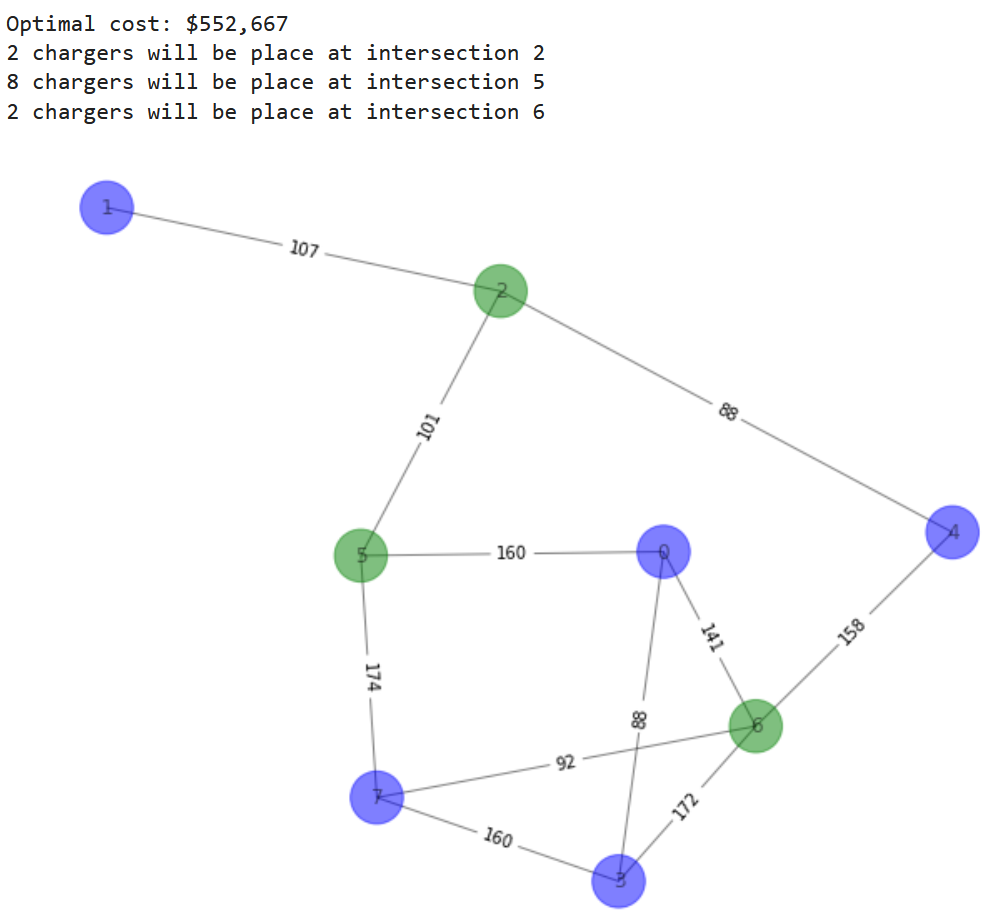
\includegraphics[width=0.6\textwidth]{model-instance.png}
\end{center}
The \textbf{green nodes in the image have charging stations}, and the \textbf{blue nodes do not have charging stations}.
An intuitive test of the model result can be seen as successful
if we consider the fact that the charging stations are spread out in the network.


\subsection{Reflection}

Since the model takes many constraints into consideration, it can be scaled to fit large sized networks.
Constraints such as the maximum number of chargers at a station limit the model, but it is required in order
to account for any unrealistic feasible solutions. This multifaceted problem takes the realistic constraints
of range into consideration in order to ensure that the model can help solve the problem in the real world.
The assumptions are justified as we have done extensive research to set them. For example, we left a minimum
buffer charge of 10 Percent as drivers will not consume the entire remaining range before recharging in the real
world. Currently, we assume that there are no wait times for the charging stations to focus on the main problem of
optimal location. This also reflects the current state of charging stations as the adoption rate of electric vehicles
is still low. Since the range of all electric cars exceeds the distance between two intersections in Ontario, we included
that assumption. Some modifications to the model could include addressing the wait times for charging stations if there is
high traffic at that specific node.


\break
\section{References}

CBC/Radio Canada. (2022, June 23). How accessible are EV charging stations across Canada? | CBC News. CBCnews. Retrieved October 21, 2022, from \url{https://www.cbc.ca/news/canada/ask-electric-vehicles-faq-1.6451121}

Costs Associated With Non-Residential Electric Vehicle Supply Equipment. (n.d.). Retrieved October 21, 2022, from \url{https://afdc.energy.gov/files/u/publication/evse_cost_report_2015.pdf}

Electric cars, hybrids and beyond. GreenCars. (n.d.). Retrieved October 21, 2022, from \url{https://www.greencars.com/?fbclid=IwAR1Lg6G58a4_p-QKY89BeyIRqL5DVX_FwIdEUmhEKdkmjPbuXeaj_Gh6Ang}

Energy consumption of full electric vehicles. EV Database. (n.d.). Retrieved October 21, 2022, from \url{https://ev-database.org/cheatsheet/energy-consumption-electric-car}

Garza, F. (n.d.). Msci 332 Tutorial 2. Tutorial.

Range of full electric vehicles. EV Database. (n.d.). Retrieved October 21, 2022, from \url{https://ev-database.org/cheatsheet/range-electric-car}

Rylan Urban. (2021, December 26). Electricity prices in Canada 2021. energyhub.org. Retrieved October 21, 2022, from \url{https://www.energyhub.org/electricity-prices/}


\break
\appendix

\section{Appendix: Mixed Integer Non-linear Model}

\textbf{Sets}
\smallskip

$I:$ Set of all intersections $i$ in the network

$A:$ Set of all lengths of feasible links $(i,j)$ between intersections in the network

$R:$ Set of all intersections $i$ of routes $k$ to traverse the network

$F:$ Set of all links $(i,j)$ of routes $k$ to traverse the network

$L:$ Set of distance to destination from all intersections $i$ of routes $k$

\medskip
\textbf{Parameters}
\smallskip

$\tau:$ Distance covered by EV using 90\% of range (100\% $\rightarrow$ 10\%)

$a_{ij}:$ Length of link $(i,j) \in A$

$e_{ijk}: \begin{cases}
        1 & \text{if EV travels on link } (i,j) \text{ in route } k \,, \quad (i,j), k \in F \\
        0 & \text{otherwise}
    \end{cases}$

$f_{ik}:$ Distance from intersection $i \in I$ to the destination in route $k \in R$

$b_{k}: \begin{cases}
        f_{0k}-\tau & \text{if for route } k,\ f_{0k} \geq \tau \,, \quad k \in R \\
        0           & \text{otherwise}
    \end{cases}$

$M:$ A very large number, much larger than any possible value in the model

\medskip
\textbf{Decision Variables}
\smallskip

$x_{i}: \begin{cases}
        1 & \text{if charging station exists at intersection } i \,, \quad i \in I \\
        0 & \text{otherwise}
    \end{cases}$

$y_{i}:$ Number of chargers installed at intersection $i \in I$

$p_{ik}: \begin{cases}
        1 & \text{if EV is charged at intersection } i \text{ on route } k \,, \quad i \in I,\ k \in R \\
        0 & \text{otherwise}
    \end{cases}$

$q_{ik}:$ Range added by charging at intersection $i \in I$ on route $k \in R$

$r_{ik}:$ Remaining range when arriving at intersection $i \in I$ on route $k \in R$

\medskip
\textbf{Cost Function}
\smallskip

\begin{equation}
    C(x) = \begin{cases}
        200000 + 10000 x & x < 3        \\
        200000 + 8000 x  & 3 \leq x < 6 \\
        200000 + 6000 x  & 6 \leq x
    \end{cases}
\end{equation}

\textbf{Objective}
\begin{equation}
    \text{MIN} \quad \sum\limits_{i \in I}{C(y_{i})}
\end{equation}

\textbf{s.t.}

\begin{equation}
    y_{i} \leq M x_{i} \qquad \forall\ i \in I
\end{equation}
\begin{equation}
    y_{i} \geq x_{i} \qquad \forall\ i \in I
\end{equation}
\begin{equation}
    y_{i} \leq 10 \qquad \forall\ i \in I
\end{equation}
\begin{equation}
    M x_{i} \geq \sum\limits_{k \in R}{p_{ik}} \qquad \forall\ i \in I
\end{equation}
\begin{equation}
    q_{ik} \leq M p_{ik} \qquad \forall\ i, k \in R
\end{equation}
\begin{equation}
    q_{ik} \geq p_{ik} \qquad \forall\ i, k \in R
\end{equation}
\begin{equation}
    r_{ik} + q_{ik} \leq \tau \qquad \forall\ i, k \in R
\end{equation}
\begin{equation}
    r_{ik} + q_{ik} = r_{jk} + a_{ij} \qquad \forall\ (i,j), k \in F
\end{equation}
\begin{equation}
    y_{i} \geq \sum\limits_{k \in R}{p_{ik}} \qquad \forall\ i \in I
\end{equation}
\begin{equation}
    \sum\limits_{i \in R}q_{ik} = b_{k} \qquad \forall\ k \in R
\end{equation}
\begin{equation}
    \sum\limits_{i \in R}p_{ik} \leq \frac{b_{k}}{\tau} + 1 \qquad \forall\ k \in R
\end{equation}
\begin{equation}
    x_{i}, p_{ik} = \{1,0\} \qquad \forall\ i \in I, k \in R
\end{equation}
\begin{equation}
    q_{ik}, r_{ik} \geq 0 \qquad \forall\ i \in I, k \in R
\end{equation}
\begin{equation}
    y_{i} \geq 0\,,\ \text{and integer} \qquad \forall\ i \in I
\end{equation}

\break
\section{Appendix: Linearized Model}
\medskip
\textbf{Sets}
\smallskip

$I:$ Set of all intersections $i$ in the network

$A:$ Set of all lengths of feasible links $(i,j)$ between intersections in the network

$R:$ Set of all intersections $i$ of routes $k$ to traverse the network

$F:$ Set of all links $(i,j)$ of routes $k$ to traverse the network

$L:$ Set of distance to destination from all intersections $i$ of routes $k$

\medskip
\textbf{Parameters}
\smallskip

$\tau:$ Distance covered by EV using 90\% of range (100\% $\rightarrow$ 10\%)

$a_{ij}:$ Length of link $(i,j) \in A$

$e_{ijk}: \begin{cases}
        1 & \text{if EV travels on link } (i,j) \text{ in route } k \,, \quad (i,j), k \in F \\
        0 & \text{otherwise}
    \end{cases}$

$f_{ik}:$ Distance from intersection $i \in I$ to the destination in route $k \in R$

$b_{k}: \begin{cases}
        f_{0k}-\tau & \text{if for route } k,\ f_{0k} \geq \tau \,, \quad k \in R \\
        0           & \text{otherwise}
    \end{cases}$

$M:$ A very large number, much larger than any possible value in the model

$d_{ni}:$ SOS2 breakpoints for each intersection $i \in I$ $\{d_{1i}=0,\, d_{2i}=3,\, d_{3i}=6, d_{4i}=10\}$

\medskip
\textbf{Decision Variables}
\smallskip

$x_{i}: \begin{cases}
        1 & \text{if charging station exists at intersection } i \,, \quad i \in I \\
        0 & \text{otherwise}
    \end{cases}$

$y_{i}:$ Number of chargers installed at intersection $i \in I$

$p_{ik}: \begin{cases}
        1 & \text{if EV is charged at intersection } i \text{ on route } k \,, \quad i \in I,\ k \in R \\
        0 & \text{otherwise}
    \end{cases}$

$q_{ik}:$ Range added by charging at intersection $i \in I$ on route $k \in R$

$r_{ik}:$ Remaining range when arriving at intersection $i \in I$ on route $k \in R$

$v_{ni}:$ SOS2 variables, $n \in {1,2,3,4},\ i \in I$

\medskip
\textbf{Cost Function}
\smallskip

\begin{equation}
    C(x) = \begin{cases}
        200000 + 10000 x & x < 3        \\
        200000 + 8000 x  & 3 \leq x < 6 \\
        200000 + 6000 x  & 6 \leq x
    \end{cases}
\end{equation}

\textbf{Objective}
\begin{equation}
    \text{MIN} \quad \sum\limits_{i \in I}{\sum\limits_{n = 1,2,3,4}{C(d_{in}) v_{in}}}
\end{equation}

\textbf{s.t.}

\begin{equation}
    y_{i} \leq M x_{i} \qquad \forall\ i \in I
\end{equation}
\begin{equation}
    y_{i} \geq x_{i} \qquad \forall\ i \in I
\end{equation}
\begin{equation}
    y_{i} \leq 10 \qquad \forall\ i \in I
\end{equation}
\begin{equation}
    M x_{i} \geq \sum\limits_{k \in R}{p_{ik}} \qquad \forall\ i \in I
\end{equation}
\begin{equation}
    q_{ik} \leq M p_{ik} \qquad \forall\ i, k \in R
\end{equation}
\begin{equation}
    q_{ik} \geq p_{ik} \qquad \forall\ i, k \in R
\end{equation}
\begin{equation}
    r_{ik} + q_{ik} \leq \tau \qquad \forall\ i, k \in R
\end{equation}
\begin{equation}
    r_{ik} + q_{ik} = r_{jk} + a_{ij} \qquad \forall\ (i,j), k \in F
\end{equation}
\begin{equation}
    y_{i} \geq \sum\limits_{k \in R}{p_{ik}} \qquad \forall\ i \in I
\end{equation}
\begin{equation}
    \sum\limits_{i \in R}q_{ik} = b_{k} \qquad \forall\ k \in R
\end{equation}
\begin{equation}
    \sum\limits_{i \in R}p_{ik} \leq \frac{b_{k}}{\tau} + 1 \qquad \forall\ k \in R
\end{equation}
\begin{equation}
    y_{i} = \sum\limits_{n = 1,2,3,4}{d_{in} v_{in}} \qquad \forall\ i \in I
\end{equation}
\begin{equation}
    \sum\limits_{n = 1,2,3,4}{v_{in}} = 1 \qquad \forall\ i \in I
\end{equation}
\begin{equation}
    x_{i}, p_{ik} = \{1,0\} \qquad \forall\ i \in I, k \in R
\end{equation}
\begin{equation}
    q_{ik}, r_{ik} \geq 0 \qquad \forall\ i \in I, k \in R
\end{equation}
\begin{equation}
    y_{i} \geq 0\,,\ \text{and integer} \qquad \forall\ i \in I
\end{equation}
\begin{equation}
    v_{in} \geq 0\,,\ \text{and of type SOS2} \qquad \forall\ i \in I, n = 1,2,3,4
\end{equation}

\end{document}